\begin{frame}
	\frametitle{Konzept}
	\framesubtitle{Ballnachführung}
	\begin{columns}
		\begin{column}{0.4\textwidth}
			\begin{block}{Ballbeschleunigung}
				\begin{itemize}
					\item Stahlband
					\item DC Motor
				\end{itemize}
			\end{block}
			\centering
			\rule{0pt}{0.8\textwidth}
		\end{column}
		\begin{column}{0.6\textwidth}
			\centering
			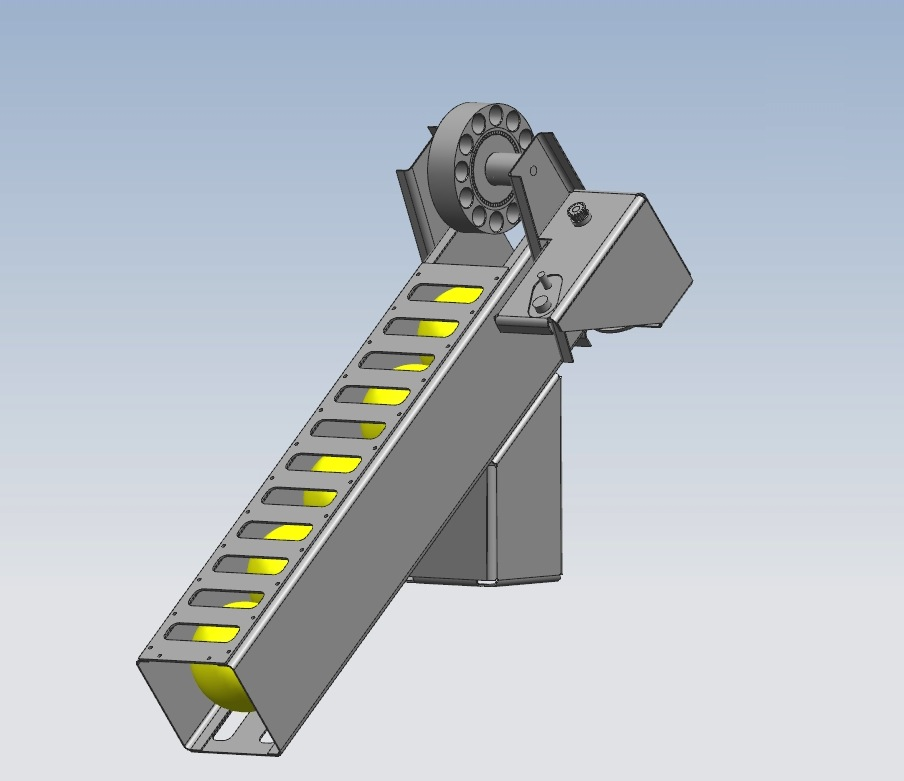
\includegraphics[height=0.8\textwidth, trim = 40mm 0mm 60mm 30mm, clip]{../doc/fig/Balllager.jpg}
		\end{column}
	\end{columns}
\end{frame}